\documentclass[10pt,a4paper]{article}
\usepackage[utf8]{inputenc}
\usepackage{amsmath}
\usepackage{amsfonts}
\usepackage{amssymb}
\usepackage{graphicx}
\usepackage{microtype}
\usepackage{parskip}
\usepackage{listings}
\usepackage{float}
\usepackage{hyperref}
\usepackage{soul}

\title{Einar's guide to better code}
\author{Einar Nyberg Karlsen}
\begin{document}
\lstset{language=Python, 
		showstringspaces=false,
		basicstyle=\ttfamily\small}
		
\maketitle

\tableofcontents

\newpage

\section{Introduction}
Hello. I am sure that you're wondering why you need to read this. You know how to code, you've coded so much during your time at NTNU. However, this is most likely not true. 

Consider a cook. If you are asked to judge how good a cook is, you would first think of whether the food tastes good, however, this is not enough. The cook should have good hygiene, know what ingredients that are used, be efficient, serve all the courses at the right time, not leave a hellish mess at the kitchen after making the food, not make a meal that is ridiculously overpriced. Coding is much the same. 

So far, you have probably only been taught how to make code that performs the expected task. Probably quite quickly as well. This is usually enough for personal sporadic use, but on a larger project, this will end up breaking the project eventually. This is why having clean code is important, as demonstrated by the graph below.

\begin{center}
\begin{figure}[H]
\label{cleanCodeEfficiency}
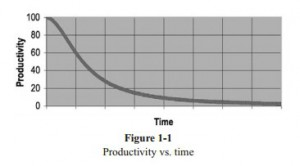
\includegraphics[scale=1]{clean-code-productivity-300x166.jpg}
\caption{A graph taken from the book "Clean Code", describing the typical productivity graph resulting from consistently writing messy code} 
\end{figure}
\end{center}

The reasoning behind this illustrative graph, is that as projects grow, more and more programmers working on it will depend on each others code, and if everyone produces code only they themselves can use, the project will halt, and work will have to be done to fix it. 

Throughout this guide, I will explain the essentials of making good code, and I urge you to read this guide in its entirety. At the end there will be a short summary and a cheat-sheet, but if you haven't read the guide, I doubt you'll appreciate the significance of the things in it. However, I will understand if you skip right ahead to it. 

A lot of the lessons in this guide are condensed snippets from the book "Clean Code" by Robert C. Martin. While I don't agree 100\% with what he claims in that book, I'd say it's somewhere between 90 to 95\% . If you have the time, I recommend reading this book in its entirety. 

Mind you, that if you choose to read the whole thing, I will often start with an example which is considered to be bad code, and incrementally make it better. Please be aware of that fact as you read through it, as some of my "solutions" are not proper solutions, but increments towards them. 

\newpage
\section{Common Problems}

So, what are the most common mistakes people make? In my personal experience, and from a fair amount of reading up on the matter, the following seem to appear a lot:

\begin{itemize}
\item bad naming of functions and variables
\item unnecessary optimization
\item no unit testing
\item The "do it all" function
\item lack of hierarchy in project
\item cross and circular dependencies
\item no documentation of work
\item inconsistent or complete lack of namespacing.
\item re-inventing the wheel
\end{itemize}


Now, if you read this list and considered all the listed issues as independent, you need this guide. For instance, having a namespacing convention in place will also cover the naming of functions. Unit testing is inherently tied into the "do it all" function, as well as hierarchy. Unnecessary optimization will also be affected by unit testing, as unit testing will allow you to monitor the behaviour of each individual module. Documentation is also tied to the namespacing, as having "function1(a, b)" will cause you to need to explain each function wherever you call it, while "vectorCrossMultiply(vect1, vect2)" will be rather self explanatory. As a matter of fact, only re-inventing the wheel is independent of the other points.

Therefore, I will split it into the most critical components of each subject, and handle each separately.

\newpage
\section{Re-inventing the wheel}
Quite honestly, this is the simplest, and the one you've most likely already have learned, but it's still good to repeat it. For any well established programming language, there are tons of libraries that do everything from file management, math, sound, etc. In our case, Python has SciPy, the scientific library containing an incredible amount of numerical and graphical tools, and it is just one of many well maintained packages out there. 

So, essentially, check first to see if the needed functionality is already implemented in the project, and if not, try to use as much from libraries as possible, as they are most likely better on performance and less prone to bugs.

\section{Conventions, and why you should adhere to them}
%TODO rewrite this shit
Isn't it wonderful how I have written all these words and you can read them and understand them fully? This is due to the English language having strict demands on things like syntax, what tense the verb is in, and so on. If talk like Yoda I do, harder for you to understand it gets. While you understood that sentence, you were probably put off a bit, because the order was quite frankly wrong. Now, I have probably made some minor syntactic or grammatic mistakes here and there, but I am still confident that you can understand me despite these minor issues. 

Writing code that others need to read is much the same, and therefore besides the programming language, there are conventions. 

The most important convention to follow is of course the convention used in the project already, assuming that it has a convention it follows. If everyone talks like Yoda, it's better to play along than to make discord. However, if 1/5 talk like Yoda, 1/5 speak Klingon, and 3/5 regular English with varying accents, you will want to stick to English yourself, get the Klingons to switch to English, then the Yodas, only then, you might want to discuss the accents.

Now, let's start with the conventions!

\subsection{Namespacing and naming your functions and variables}

The most important convention of them all. Because this is very much tied into how you write your code, how you understand it, and how everything in it ties together.

Allow me two examples:
\begin{lstlisting}
from bigFileWithManyFunctions import *
from numpy import *

def main():
	var1 = 15.1
	var2 = 12.3
	var3 = 2.5
	var4 = area(var1, var2)
	var3 = degrees(var3)

\end{lstlisting}

Now, this is not easy code to read. As you can see, you have no concept of what the variables are, you can't intuitively see whether area and/or degrees comes from the bigFile... import, or the numpy import, as both import to the global namespace. Further, if any function in bigFile has the same name as a function in numpy, the numpy function will be the one to be called as it was imported last. This is extremely problematic as it makes the code prone to errors that can be hard to track down. Let's now look at some better, but not good, named and namespaced code.

\begin{lstlisting}
import bigFileWithManyFunctions as bigFile
import numpy as np

class RectangleWithTemperature(object):
  def __init__(lenX, 
               lenY, 
               tempFahrenheit = 60, 
               printCompletion = False,
               boolConvToCelsius = False):
               
    self.lenX = lenX
    self.lenY = lenY
    self.area = np.area(lenX, lenY)
		
    self.t = tempFahrenheit
    if boolConvToCelsius:
      self.t = bigFile.degrees(self.t)
    
    if printCompletion:
      print "construction of rectangle complete"

def main():

  rectInstance = RectangleWithTemperature
                 (lenX = 15.1, 
                  lenY = 12.3, 
                  tempFahrenheit = 2.5, 
                  convToCelsius = True)
	
\end{lstlisting}

One thing worth noting here, is that you probably thought that degrees referred to angle, which is what it normally does. However, the coder here has been naughty, and not properly named his function "degrees", which should have been called "convFahrenheitToCelcius". And, to make matters worse, the function even had the same name as the numpy function degrees, which converts radians to degrees. So, not only was the original code unorganized, it was also wrong because of bad imports.

You're thinking that I'm belittling you right now, but there is a very good reason why I'm pushing for you to be pedantic about this. At some point, your module will be complete, and you will jump over to working on another one. Then, half a year later, someone else encounters a bug coming from your module. He tries to find the bug, but can't understand the error message, so he contacts you. The problem is, you haven't looked at that code for half a year. You don't remember much of it, so you start looking at it again. What made sense half a year ago might not make sense any longer, and you're as stuck as he is, and late shifts of debugging the code ensue for the both of you. 

One final thing to notice, is how in the improved version, I call the class with parameter names as well as values. This is due to the fact that I have here hard-coded the values into the function call, and just seeing a list saying "15.1, 12.3, 2.5, True" won't say much to anyone looking at the code, and they'll have to look up the class constructor to see what the parameters mean. A general rule to consider is that if you need to look up the function's documentation to see what the parameters it's been called with mean, you probably want to use the parameter names in the function call. Further, in Python, using the parameter name will allow you to choose specific optional arguments, which can simplify a lot of function calls.

\subsection{Commenting your code}
While having reasonable names will make your code a lot cleaner, it is close to inevitable that the code reaches a point where you can't easily understand it just from looking at it. There are tech companies that claim the contrary, like Cisco, but they're highly skilled and enforce extremely strict structural conventions. Thus, we regular human beings cheat a little: we comment our code. 

Throughout this project, there are two types of commenting, the regular \# commenting, which is to be used for those looking to inspect or modify the code directly, and docstrings, which are started and ended by triple doublequotes. Docstrings are to be used to document the code, and should be placed on each callable function, explaining shortly what it is intended to do, what parameters(inputs) it expects, and what it outputs. Essentially, it should explain the utility of a function, but not its inner workings, a "black-box" description of the function. For our project, we adhere to the google docstring standard.

Let's look at how the code looks with even better names and a bit of commenting.  

\begin{lstlisting}
import rectangleUtilities as rectUtils
import numpy as np

class RectangleWithTemperature(object):
  def __init__(lenX, 
               lenY, 
               tempFahrenheit = 60, 
               printCompletion = False,
               convToCelsius = False):
    """
    Initializes an instance of rectangleWithTemperature
    
    Args: 
      lenX (float): length in X direction in meters
      lenY (float): length in Y direction in meters
      tempFahrenheit (optional float): 
        temperature in Fahrenheit, defaults to 60
      printCompletion (optional bool):
        decides if constructor will 
        print success upon completion.
      convToCelsius (optional bool): 
        decides whether or not to set temperature 
        in Celsius, defaults to False.
    """
    
    # initialize lengths
    self.lenX = lenX
    self.lenY = lenY
    
    # initialize area
    self.area = np.area(lenX, lenY)
	
    # initialize temperature variable
    if convToCelsius:
      self.temp = rectUtils.convFahrToCelcius(tempFahrenheit)
    else:
      self.temp = tempFahrenheit

    # print success    
    if printCompletion:
      print "construction of rectangle complete"


def main():

  # initialize rectangle instance
  rectInstance = RectangleWithTemperature(
                  lenX = 15.1, 
                  lenY = 12.3, 
                  tempFahrenheit = 2.5, 
                  convToCelsius = True)
	
\end{lstlisting}

Now, if anyone looks at the code you've written, they will see that they need to give the input lengths in meters, which would not really be intuitive as the temperature was given in Fahrenheit. While you might think this won't be a problem, "everyone uses meters and Celsius", a lack of clarity and strictness on such issues has actually caused space-shuttle launches to fail. And besides, they might use Kelvin instead of Celsius. Clarity on input, output, and expected error messages and will save you personally some minor trouble, but can save the group working on the project a whole lot of trouble. 

Also, as you can see, thanks to the good naming of variables and functions, all of the hashtag comments are unnecessary. You can understand every part of the code by just looking at it. Which brings me to my last point when it comes to commenting, stolen from the book Clean Code mentioned earlier.

Commenting should be considered a last resort to fix the failure of the code to be self-explanatory.

Of course, this is a bit strict, There might be frameworks that won't allow us to make neat code, or some other valid reason. So, don't feel bad about having comments, but try to always keep it in mind, that the code should be readable without it to the best of your ability. A good way to code is to first write the comment, implement, and see if you now can remove your comment and it's still understandable. If you can't, you should really take a long hard look at whether or not you need to re-factor it. And most importantly, if you can't avoid having a comment, make sure your code actually does what your comment says it does. Few things are more time consuming than a bug hiding behind a misleading comment. 

Docstrings however, should always be used, as these will be read by our auto-documentation script, and will provide the foundation of our API documentation. (The docstrings in this guide might be slightly wrong, as showcasing code in latex forces a slight reordering of lines.)

\subsection{The conventions we use in our project}

First off, we try to be compliant to the \href{https://www.python.org/dev/peps/pep-0008/}{PEP-8 standard}. The most important parts to know is the following:

\begin{itemize}
\item Use 4 spaces, not tabs (you can get your editor to do this automatically, and it is in recommended for coding in general).
\item If your function has many inputs, list them vertically by having an extra indent or more. See the code example above how rectangleWithTemperature is called if you want an example.
\item We use CapitalizedWords and mixedCase mostly in our code. We capitalized the first letter to signal that this is a class, and we keep it in lowercase if it is an instance of a class, or a function. This allows us to easily see what we're working with.
\item We disobey the convention on function names, where PEP 8 wants them to be lowercase and seperated by underscores, we use mixedCase for functions as well. This is due to underscore being a hassle to use.
\item If you have a list of things, add list to the name. Do not use plural s. \\
good: vesselList, bad: vessels
\item Further, as we have a project with a lot of functional files, we often use the "import .... as .." method, where we have a list of abbreviations that you are expected to follow.
\end{itemize}

Now, there is one important aspect of this that you need to know. This code base is a work in progress, the conventions are not necessarily implemented thoroughly at the moment you're reading this. This means that some times, you might have to break the conventions to make it work with the existing codebase. However, this should be the only time when you break the conventions we have set for this project.

However, we are working hard to re-factor the code to be compliant with the conventions, unit testing and exception handling. If there is no compatibility concern, you should always comply with this guide, not the codebase. In the case of exception handling, always comply to this guide.

Throughout the guide, there will be a lot of code used as example. However, a lot of it will intentionally be sloppy, so it can showcase the issues with sloppy conventions and methodology. If in doubt, check the Cheat Sheet at the end of the guide for correct conventions.

%TODO nevn hvilke filer som har brukne imports. 

\newpage
\section{Hierarchy, or why size matters}

I want you to consider a machine. Consider all the parts it's made of. Consider how most of those parts are rather standardized. They are of a specific form, attach in a specific way, and perform in a specific manner. Each component has certain demands in functionality and structural integrity. Programs are much the same. In any large program, if you "pop the hood" on it, you will almost always find that it consists of smaller programs working in conjunction, just like any machine would. And, just like you wouldn't want to design a machine without splitting it into components, the same applies to programming. 

\subsection{Abstraction levels}
Now, The programmer who wrote Clean Code says that functions should stay within one abstraction level. In the case of numerical programming, I find this to often be too strict, as the nature of numerics often demand a few layers of abstraction co-existing. But, as always, he's not that far off either. The more you can split things up into simple operations, the more control you have. Let's make an example to illustrate how it works.

\begin{lstlisting}

def moveRightLeg(directionClass):
  moveRightLegSideways(directionClass.side)
  moveRightLegAlong(directionClass.along)
  moveRightLegHeight(directionClass.height)

def moveRightLegSideways(sidedata):
  if sidedata == 0.0: return None
  elif sidedata < 0.0: # to the left
    moveRightLegLeft(abs(sidedata))
  else:
    moveRightLegRight(sidedata)

\end{lstlisting}

And so it continues. This might seem a bit pedantic, but imagine the incredible amount of code that would appear in moveRightLeg if you didn't abstract it into smaller functions. Of course, there are times when functions are inherently connected, and you can't avoid it. 

As you can see in this mock-code, it is really simple to understand what the function does in rough detail. You will have to inspect the deeper functions, to see the inner workings, but do you really want to do that for all the code you will use? Thus, I present the black box.

\subsection{The infamous black box}
I want to introduce a concept that is important to any programmer, engineer and scientist, but is very often overlooked. The concept of the black box. The simple definition of a black box is a system where a set of inputs produce a set of outputs according to the logic of a obscured mechanism. In other words, that it's a system where it's easier to consider input - output, rather than how it actually works. 

\subsection{The + sign, a beautiful black box}
I want to ask you now, what happens when you ask python to do c = a + b ? You don't really think about it, but it's a lot more than you first think. First of all, it compares the types of the two, if they're the same, it calls the + function of the type of a, with b as its argument. If they're not, it has to look deeper, for instance, if a is an int, and b is a float, then it'll convert a to float, and then add them using float.add. However, if one of them is a string, then the two types are incompatible, and it raises a TypeError. And then you have the really deep mechanisms of how it works physically in the processor again.

Why did I just tell you all of this? Because I want you to consider how much the single "+" sign actually does in python, and how few people really have considered that fact. This is the hallmark of a good black box. And now comes the morale of all this: Everything you program in a project will at some time become a black box. 

\subsection{Design black boxes, not white ones}
At some point, the module will be considered complete, and you'll move on. Then a year goes by, and you need to look into your old black box because it seems to be the root cause of some weird bug. Now, if you have been good with naming, namespacing and commenting, and made sure that your exception handling is adequate, you will be able to open up your old black box and inspect the mechanisms in a fairly short amount of time, and fix the problem. 

However, it might be that the problem isn't the box itself, but its description. The most important reason why I want you to consider all code you write as a black box, is for the sake of others. If your black box is well defined, with strict input, output, and exception handling, other programmers will be able to use it as a black box. This allows them to employ your work without having to inspect and understand the foundation of your program. They might want to anyway, but they won't have to. This increases productivity a lot. 

\newpage
\section{Exceptions, friend or foe?}

You've probably seen this a hundred times, you have a typo, pass the wrong parameter, and the program dies with an error log that gives a bunch of tracebacks and a certain kind of error, like "TypeError: object [int] has no attribute append". While your previous experiences with exceptions might be that they are rather unhelpful, with some care, they will be your allies in debugging, and you should use them for all they're worth. 

\subsection{The road to success is paved with failures}

Wait what? You want me to fail?

Well, not exactly. I want you to cause your code to fail in every possible way. If you have a code that should open an XML file, I want you to test giving it a txt file. I want you to test giving it a python file. I want you to test giving it a file that doesn't exist. I want you to test giving it a corrupted file. You get the picture. And I want you to keep those tests for later, I'll gea padded message,t back to that in the next section. 

Essentially, sooner or later, you, or someone else, will mess up, and use your code in the wrong way. When that happens, you want your code to give as specific and useful information as it can, because the standard error messages are less and less useful as the project grows in size.

Let's construct a hypothetical scenario:
you have a main function that calls on moduleReadFile 100 times to read 100 different files. It then passes the output from moduleReadFile to moduleProcessFileData, which in turn depends on 3 submodules. 

The standard error message you will get is something along the lines of this: 

\begin{lstlisting}
Traceback (most recent call last):
  File "Main.py", line [last line] in <module>
    main()
  File "Main.py", line X in main    
    moduleProcessFileData.process(outputFromMRF)
  File "moduleProcessFileData line Y in process
    submodule2.sanitize(line)
  File "submodule2",  line Z in sanitize
    splitInput = inputLine.split(".")
  AttributeError: 'NoneType' has no attribute 'split'
\end{lstlisting}

Okay, so you have an empty line or something being passed on. Which file did it come from? the first, last? one in the middle somewhere? We want our program to catch exceptions, process them, and pass them on, and in python, this is called "try:" and "except (optional: exceptionType):"

Let's say we now add some cheap information to the program. We encase line X in the following way:

\begin{lstlisting}
  for filename in filenamelist:

    #read file
    try:
      outputFromMRF = moduleReadFile.read(filename)
    except:
      print "failure reading {}".format(filename)
      
    # process file
    try: 
      result = moduleProcessFileData.process(outputFromMRF)
    except: 
      print "failure processing {}".format(filename)
\end{lstlisting}

Now we'll get information about the filename that is useful when the program crashes, but unfortunately, our files are thousands upon thousands of lines, and we can't efficiently process them. So we want to have something in moduleProcessFileData to fix that.

\begin{lstlisting}
numLine = 1
for line in inputFileData:
  try: 
    submodule2.sanitize(line)
    numLine = numLine + 1
  except:
    print "Error when using submodule2.sanitize(line) 
           with line number {} from file".format(numLine)

\end{lstlisting}

Now we're getting somewhere. We run the program, but it's no good. We get the error, and it prints the line number, but the error message stops there.

This is because "except:" catches everything. Not only will it now not send errors to the main function, but it will also keep working. This can cause your code to pass on bad data to the next submodule, which will crash because of an error in the previous one. This is why we will always want to re-raise the exception, using the simple command "raise"


\begin{lstlisting}
numLine = 1
for line in inputFileData:
  try: 
    submodule2.sanitize(line)
    numLine = numLine + 1
  except:
    print "Error when using submodule2.sanitize(line) 
           with line number {} from file".format(numLine)
    raise

\end{lstlisting}

Now the function will get the error message, print out relevant information, and pass the exception along to the main function, which can then print out its information, and we should put a raise on the main function as well, as we don't want our program working on potentially corrupt data, and we rather want it to die before it does any harm. 

For instance, you might find that it says it failed on the 54. file, line 1, which is a good indicator that the file is either empty or corrupt. Having this information would be impossible without the exception handling, or a debugger, but debuggers are a hassle to use in my opinion, and it's better to actively counteract such problems than to rely on a tool to fix them retroactively.

So, the quick lesson for the most rudimentary exception handling is as follows:

\begin{lstlisting}
try: 
  stuff(parameterlist)
except:
  print "Error in function stuff with parameters {} 
         ".format(parameterlist) 
  raise
\end{lstlisting}

Using this method consistently will cause your program to always give reasonable error messages. However, there are times when you want to handle your exceptions.

\subsection{Exception handling}

Now, the method I ended with on the last subsection was good for giving good feedback when your program crashes and burns, but it neglects one scenario: When you expect your program to fail some times, and want it to continue just the same. 

That should be simple shouldn't it? All we do is that we don't raise the exception again.

\begin{lstlisting}
try: 
  stuff(parameterlist)
except:
  doStuffToHandleException(parameterlist)
  print "Warning: doing stuff with parameters {} 
         failed ".format(parameterlist) 
\end{lstlisting}

There, all done! let's take the day off!

or not...

Because, it turns out that the clause "except:" does 
not only stop exceptions, but also keyboard and system interrupts. 
This means that if your program has bloated to the point it's crippling your computer, and you want to stop it, it will ignore the nice system calls, and you will have to kill the process with an axe.

As you can understand, this is unwanted behaviour, and we need to fix this. The first instinct would perhaps to append the code executed within the except clause with some tests, but this will cause the except clause to be ugly and unruly.

When you want to handle your exceptions, the first step is finding out how your module fails, and that it fails when it should. Using this information, you should in a project be able to know whether you're expecting a TypeError, NameError, or some other exception class, based on what you except the function to do. 

Let's look at a modified version of the last attempt.

\begin{lstlisting}
try: 
  stuff(parameterlist)
  
# expected type of error, will be cleaned out and ignored.
except TypeError as e:
  handleTypeErrorExceptionInStuff(parameterlist)
  print "Warning: doing stuff with parameters {} 
         gave TypeError with following message:
         ".format(parameterlist)
         print e 
         print "Parameter list should consist of 
         types {} ".format(idealParameterlist)


# expected type of error, should kill program unless 
# ignoreUnimplemented == True
except NameError as e: 
  if ignoreUnimplemented == True:
    print "Warning: stuff with input parameters {}, 
           wanted to call function that is not 
           implemented".format(parameterlist)
    print type(e)
    print e
  else:
    print "Error: stuff with input parameters {}, 
           wanted to call function that is not 
           implemented".format(parameterlist)  
    raise

# Any other kind of exception
except Exception as e:
  print "caught unexpected exception in function stuff
         with parameters {}".format(parameters)
  raise
  
\end{lstlisting}

As you can see, now we will handle a TypeError and allow the program to progress, while we will let the NameError's handling be determined by a boolean. And any other Error messages will be called out as unexpected. Perhaps most importantly is to notice that the NameError's handling raises the exception out of the scope of the try-except clause, so that except Exception does not catch it.

Another very important thing to notice, is that this will not catch system errors and calls. System errors will propagate all the way and kill the program, which they should. 

Of course, I'm being overly descriptive in my warning and error messages in this code, real code will not need this level of pedantic error messages, but you will find that I'm not that far off either. 

\subsection{How to actually do it}

I'm a bad person. I've shown you so much, and it's not actually they way you're supposed to handle exceptions. Before you get angry, please bear with me. The reason I've shown you this is because it's easier to explain the logic before introducing the concept of padding your exception. Let me show you how it's actually done.

\begin{lstlisting}
try: 
  stuff(parameterlist)
except Exception as e:
  raise type(e), type(e)(e.message + 
                  '\n IN FILEA: function stuff was called with 
                  params {}'.format(parameterlist)), 
                  sys.exc_info()[2] # traceback info
\end{lstlisting}

As you can see, we don't print anything, instead we raise a new exception that has the same type, the old message appended with new information, and contains the original traceback. This has certain advantages. First of all, you can decide at any level whether or not the message should be silent, whereas with the print method, you will always print each step until you reach the one that suppresses the exception. Secondly, you will get the whole string in one piece, at the end of your error traceback, which means that you can look at it the same way you would a standard unhandled exception. Third, and maybe the most important, this allows for neater unit testing, as print statements are not particularly liked by python's unit testing framework. 

However, and this is important, you should still consider having print statements, or some error/warning logging for the exceptions that do get suppressed.

\subsection{The other types of exceptions}

I will urge you to look at this webpage, \href{https://docs.python.org/2/library/exceptions.html\#exception-hierarchy}{Pythons exception hierarchy} to get a general idea of how exceptions are structured. As you can see, there are three classes beside Exception. There's SystemExit, KeyboardInterrupt, and GeneratorExit. 

\begin{itemize}

\item SystemExit covers calls to sys.exit(), which can be called within the code, or be injected by the OS when you wish to terminate the code. If your exception handling catches these, it should only be to allow it to die neatly, or give a logfile of what it was doing before terminating. Any call to these functions should result in your code terminating. os.exit() will not be covered by this, as this is the kill command, which essentially just tells your code to terminate as quickly as possibly. It should in principle be treated the same as a KeyboardInterrupt.

\item KeyboardInterrupt is rather self explanatory, you run your program, but want it to stop, you press ctrl-c. Only ever catch this if you need to avoid data corruption before terminating your program. And, if you do this, add a print statement that allows the user to see that the interrupt has been registered, and that the program is cleaning up before terminating.

\item GeneratorExit is actually not really an error or an exception. However, because you might want to perform certain actions when closing a generator, they added this to the built-in exceptions so it would have the desired traits. Unless you're using a generator, you will not need to bother with this one.

\end{itemize}

As you can understand from this list, Exception is the one you want to focus on. However, since I've already spent so much time explaining it, I'll just say this final thing: Notice that Warning is a subclass of Exception. This is because the functionality of the Exception class is suited for Warning. But, when issuing warnings, one uses warnings.warn(Warning('text')), as this does not start the termination chain a regular Exception would. The rest of the Exception tree should be self-explanatory enough. 

\newpage
\section{Unit Testing and You!}

%TODO fix overselling, refactor into having own chapter on blackbox etc.
Now comes the juicy part: unit testing, and why this will cause you to write better code, implement a good hierarchy, avoid using time on unnecessary optimization, and most importantly, avoid the big taboo, having just one big blob of a function.

\subsection{What is unit testing}
So, what is unit testing? Simply put, unit testing is the method of always testing what you implement before moving on. Now you're probably thinking "but I already do that", and you're probably right, but do you keep the tests? Are they structured, do they test all demanded behaviours, including how it handles wrong input? If you have a function that should add two vectors together, what happens if they are of different lengths? what if one consists of integer values, the other floating points? 

This is why you want to build unit tests for each module you make. Mind you, I'm not talking about checking if 2 + 2 = 4, some things you should assume just works, but rather, I want you to have a clear idea of exactly what should happen when you input parameters into your function, what it returns. As we will be working on numerical simulation, runtimes will be dominated by the numerical solvers, which means that until the program is complete, optimization of anything else will not be a priority. However, knowing how each module behaves will be, and if you recall Figure \ref{cleanCodeEfficiency}, it is crucial to the project's progress. 

If you do unit testing correctly, it'll be \href{http://stackoverflow.com/questions/61400/what-makes-a-good-unit-test}{"A TRIP"}.

\subsection{What testing paradigm is best for you?}

Essentially, one decision you have to make, is the following: Tests first, then code, or code first, then tests? This is actually not clear cut, as both have advantages and disadvantages. 

Tests first, or Test Driven Development (TDD) as it's called, has the advantage of forcing the programmer to structure the code in beforehand, and have set forth a very clear set of goals before implementing them. The problem with TDD is that it can often be felt as crippling the flow of production, as you regularly have to stop to construct the tests, and it can be really hard to have a clear feeling of what exactly should happen before you've actually implemented it. Of course, the latter argument is as much an argument against TDD as it is in favour of it.

However, code first, tests later is more in touch with the standard way of doing things. The most obvious pitfall of this approach is the danger of forgetting tests altogether, which is bad. Further, it allows you to stay more in the flow while programming, which can both be beneficial, as your productivity will be high, but also detrimental, as you might produce a lot of code that will need refactoring once you start testing it. The advantages and disadvantages when it comes to the tests themselves is that you will have an easier time knowing what wanted behaviour to test, but you can also have a harder time constructing tests concerning unwanted behaviour. 

My personal recommendation is simply to try both. Some will want to force themselves to test thoroughly by adhering to TDD, while others will want the freedom to do it a bit more at their own pace.

But make no mistake, you should test your code, and you should do it properly, using either the built-in features of python 2.7, or an extended testing library. For this guide, I will focus on the built-in, as most of the extended ones are built upon it again. 

\subsection{The unittest package}

Now, Python has a built-in library, unittest, which will help automate a lot of the testing. The standard procedure is as follows:
\begin{enumerate}
\item import unittest
\item import file(s) you wish to test
\item make class(es) which inherit from unittest.TestCase
\item make functions within the classes with the name test\_whatYouWishToTest. Use self.assert[type]() calls within the function. \href{https://docs.python.org/2/library/unittest.html\#unittest.TestCase.debug}{List of asserts}
\item end with the following line: \\
 if \_\_name\_\_ == '\_\_main\_\_': unittest.main()
\end{enumerate}

Enough dry talk, let's have an example.

\begin{lstlisting}
import unittest
import FileToTest

class TestStringMethods(unittest.TestCase):

  def test_splitString(self):
    s = 'hello world'
    self.assertEqual(FileToTest.splitString(s), 
                     ['hello', 'world'])
    with self.assertRaises(TypeError):
        FileToTest.splitString(2)

if __name__ == '__main__':
    unittest.main()

\end{lstlisting}

Now, as you can see, it's fairly straight forward, your class inherits from the TestCase class in the unittest package, so that it contains specialized assert functions used by unittest.main(). All tests are in functions prefaced with test[underscore] and a descriptive name. But, there are certain issues with this test. 
First off, if test\_splitString fails, you will have to look at what part of the test itself failed. This is why it's common practice to split tests into as simple as possible tests. 

However, it might be that you want to have several tests that want to use similar variables. But, as was mentioned in the acronym "A TRIP", one important criteria is the independence of tests. The way to solve this is by abstracting the tests into having inheritance themselves.

\begin{lstlisting}
import unittest
import FileToTest 

class SetUpStringTestCase(unittest.TestCase):
  def setUp():
    self.testString = 'hello world'
    self.correctSplitString = ['hello', 'world']
    self.wordCount = 2
    self.letterCount = 10
    self.spaceCount = 1


class TestSplitString(SetUpStringTestCase):

  def test_correctBehaviour(self):
    self.assertEqual(FileToTest.splitString(self.testString), 
                     self.correctSplitString)

  def test_wrongInputType(self):
    with self.assertRaises(TypeError):
      FileToTest.splitString(2)

  def test_tooManyArgs(self):
    with self.assertRaises(TypeError):
      FileToTest.splitString(self.testString, 
                             self.testString)


class TestConcatinateString(SetUpStringTestCase):

  def test_correctBehaviour(self):
    self.assertEqual(
        FileToTest.concatinateString(self.correctSplitString), 
        self.testString)

  def test_wrongInputType(self):
    with self.assertRaises(TypeError):
      FileToTest.concatinateString([1, 2])
          
if __name__ == '__main__':
    unittest.main()

\end{lstlisting}

As you can see, this way, each class will specify what function you wish to test, and each testing function will specify what aspect you wish to test. Further, each test case will initialize a standard set of values defined in the SetUpStringTestCase class, so you won't have to initialize those variables over and over. Further, by adhering to the naming and namespacing conventions, the code is quite self-explanatory.

Now, there is one huge pitfall in this code. If for instance, in class TestConcatinateString, test\_correctBehaviour changes one of the variables, that change will carry on to the next test in the class. So be careful, and if in doubt, split the tests you suspect can change the variables into their own classes. However, since we're working in Python, it's less likely to be a problem than in languages that depend more on call-by-reference.  


\subsection{Unit testing, slayer of dragons}
Now, as you might have thought; "But I can't devise a test for my bigFunc(inp1, inp2, inp3, inp4, etc etc), what should I do?". The simple answer is: don't make bigFunc.

What? But I need bigFunc! Or so you might think. But it actually makes sense. No matter how complex your operation might seem, it will almost certainly consist of smaller tasks. And, rather than clustering them together, separate them. Essentially, it boils down to a simple message: if it's too big to unit test, it's too big to exist.

This is why I call unit testing the slayer of dragons, because big black boxes with unpredictable behaviour are like dragons, pretty at first, deadly when poked in the wrong spot. However, apply a regime of unit testing to your development process, and you'll find what functions are too big without looking specifically for them.


%\subsection{Making mock functions for testing}
%TODO decide if should remain


\subsection{Systematising your tests}

Now, how should your tests be? Let's reference Clean Code again by looking at another acronym: FIRST.

\begin{itemize} 
\item Fast. Let's look back at the case I used to illustrate the need for exceptions. A function that would take in 100 files, feed each file into another function. To test that, you only need to feed it two files, that can be empty for all it cares. As a matter of fact, because it asks the moduleFileRead for the actual reading, the test doesn't even have to check that it reads the files, only that it calls moduleFileRead.readFile() with the elements from its input list. Similarly, you only have to test that it then takes whatever output, as long as its not an exception, and passes it to the processing module. The general rule is that your tests should be minimal.
\item Independent. This is the most important one. Every test should test one thing, and one thing alone. If your function should switch between three different outputs depending on its input\footnote{Well, if it does, you really should look into refactoring your function, but this is just for the purpose of demonstration.}, then you should have three separate tests to check that all three work. They should not depend on the result of anything else. This is important because you need to be absolutely sure that something fails or passes solely on its own merit. And most importantly, no test should be affected by any other test!
\item Repeatable. This one is fairly simple, you want to have your all your tests run by a single python script which uses the built in "unittest" package. I'll get to that after this list.
\item Self Validating. The tests should have a boolean output. Either the test succeeds, or it fails. This is a crucial part of making them fast as well, as it won't matter if the test runs in 0.1 seconds, if you have to spend 5 minutes to look at it to check if it succeeded.
\item Timely. This comes back to the testing paradigm. The test should be written at a relevant point in the development cycle. The way I like to think of it is that it's debatable whether or not to write tests or code first, but the test always comes before the deployment of the module. Essentially, before your code gets introduced into the project, it has to have been tested thoroughly.  
\end{itemize}

Of course, since we're programming a heavily numerical system, there's one more aspect which I'd like to stress, and it's really about thoroughness. Because of our dependence on floating point operations, which can produce rounding errors when close to zero, we want to test feeding our system edge cases that checks how our functions handle numbers close to or equal 0 whereever it's relevant. In computers, you can get that items that should have been zero actually have a microscopic value, and if they're subtracted from a number that is zero, this can lead to unwanted behaviour later in the simulation. 

Between the two acronyms, I feel that most of the testing philosophy should be covered. Of course, the topic of unit testing is so deep that many would argue it deserves its own book. But, I hope this has helped

\newpage
\section{The Short Summary}
Now that you've gone through the guide, let's recap quickly.

\begin{itemize}
\item Try to use pre-existing solutions rather than implementing your own.
\item Have clear names and use proper namespacing in your code. 
\item Document your code with docstrings adhering to the Google docstring standard. Be clear on the input-output.
\item Structure your code so that it is as self-explanatory as possible, and use \# comments where additional clarification is useful.
\item Remember that all code you write will end up being treated as a black-box sooner or later. So make sure that it actually works like one, with a clear input-output dichotomy. 
\item Exceptions should crash your program, unless you have very specific reasons why it shouldn't.
\item If you absolutely want to stop exceptions, you should not use "except:", as this will catch system exits and keyboard interrupts. If you want a catch-all, use "except Exception as e:"
\item You should catch, append and then re-raise the exception at each level of the code, so that an informative traceback will appear when the program dies.
\item Unit Testing is desirable, and you should test crucial behaviour of each feature you wish to push to the main project. Also, test that you code fails the way it should. Few things are as hard to track down as code that passes wrong data onto other parts in the program.
\item Keep your Unit tests. Write them well. Systematize them. Make sure they're thorough, independent of each other, and fast.
\end{itemize}

\newpage
\section{The Cheat Sheet}

\subsection{Conventions and Namespacing}
%TODO fix litt her
\begin{lstlisting}
import numpy as np
import UtilityLib.rectangles as rectUtils

class Rectangle(object):
  def __init__(lenX, 
               lenY = 1.0) 
    """
    Initializes an instance of Rectangle. 
    Will attempt to convert input to floats.
    
    Args: 
      lenX (float): length in X direction in meters
      lenY (optional float): length in Y direction in 
        meters, defaults to 1.0
    Raises:
      TypeError: If lenX or lenY can't be converted to floats.
      AssertionError: If lenX or lenY == 0.0.
    """
    
    self.lenX = float(lenX)
    assert self.lenX != 0.0
    
    self.lenY = float(lenY)
    assert self.lenY != 0.0

    self.area = rectUtils.calculateArea(lenX, lenY)

  def get_lenX(self):
    """Returns: float: The value of lenX """
    return self.lenX

def main():

  # construct instance of Rectangle class
  # notice naming the arguments of the constructor 
  # as they're not intuitive without the names.
  rectInstance = Rectangle(
                  lenX = 15.1, 
                  lenY = 12.3)
	
\end{lstlisting}

\newpage
\subsection{Exception Handling}

\begin{lstlisting}
try: 
  rectInstance = Rectangle(parameterlist)

# handle expected TypeError because of reasons.
except TypeError as e:  
  handleTypeErrorInRectangleInit(<relevant parameters>)
  storeHandledExceptionInfo(e, "describingString")
  
# state dependent exception handling
except AssertionError as e: 

  if allow1dRect:     # Enabled when bugtesting module. 
    handleAssertionErrorInRectangleInit(<relevant parameters>)
    storeHandledExceptionInfo(e, "describingString")

  else:               # Default, re-raises AssertionError.
    raise type(e), type(e)(e.message +       # keep old message
                    "\n "describingString"), # add new info
                    sys.exc_info()[2]        # traceback info
  
except Exception as e: 
  raise type(e), type(e)(e.message +       # keep old message
                  "\n "describingString"), # add new info
                  sys.exc_info()[2]        # traceback info
\end{lstlisting}
Of course, usually you want to only use the last part unless you have a really good reason to do otherwise. One of the most common reasons is in the case of user input, where you have to account for the user misspelling things.

Further, The handle[...] and store[...] functions are just thought up examples, if you need them, implement them.

\newpage
\subsection{Unit Testing}

\begin{lstlisting}
import unittest
import FileToTest 

class SetUpTestDataForFileToTest(unittest.TestCase):
  def setUp():
    self.correctVariable = <suitable data>
    self.wrongVariable = <unsuitable data>
    self.myClass = MyClass(<initdata>) 
    
#  def tearDown(self):  
#    self.myClass.destructor()  
#    self.myClass = None
# should be used if setUp initializes class  
# instance which needs a destructor.


class TestSpecificFunction(SetUpTestDataForFileToTest):

  def test_correctBehaviour(self):
    self.correctResult = <correctResult>
    self.assertEqual(
        FileToTest.specificFunction(self.correctVariable), 
        self.correctResult
        )

  def test_wrongInputType(self):
    with self.assertRaises(TypeError):
      FileToTest.specificFunction(self.wrongVariable)


if __name__ == '__main__':
    unittest.main()

\end{lstlisting}

\end{document}
















